\documentclass[11pt]{report}
\usepackage{blindtext}
\usepackage[margin=1in]{geometry}
\usepackage{graphicx}
\usepackage{booktabs}
\usepackage{verbatim}
\usepackage{pdfpages}
\title{Thanks Corporation Database Project\\CMSI 486 Enterprise Project\\Fall 2014}
\author{Edward Bramanti}
\date{This project designs and implements a database for an employee recognition system for companies to use internally.}

\providecommand\phantomsection{}
\newcommand*\rot{\rotatebox{90}}


\renewcommand\thechapter{\Roman{chapter}}
\renewcommand\thesection{\thechapter.\arabic{section}}

\usepackage{tocloft}
\setlength{\cftchapnumwidth}{3em}
\setlength{\cftsecnumwidth}{3.5em}
\setlength{\cftsubsecnumwidth}{4em}

\begin{document}
\clearpage
\phantomsection
\addcontentsline{toc}{chapter}{
    \protect\numberline{I}Title Page}
\maketitle
\clearpage
\phantomsection
\addcontentsline{toc}{chapter}{
    \protect\numberline{II}Table of Contents}
\tableofcontents
\setcounter{page}{2}
\setcounter{chapter}{2}
\chapter{Description of the Enterprise}

\indent Thanks is an effective, entirely digital, multi-purpose employee recognition system. The database will consist of many different companies who will pay for a service that makes recognizing employees simple and meaningful. This will allow the Thanks database to be used in a way that is unique to each company using the service.

\indent The enterprise in question will make it much easier for employees to recognize one another across their company. As companies grow, it becomes difficult to maintain an atmosphere of employee worth. This growing size represents a problem as individual employees can feel like their work goes unnoticed in their company. “Thanks” provides a remedy for that by providing a digital way to send recognition to any employee quickly.

\indent When opening the thanks form, it will be necessary to present a list of all employees in the company. A list of employees would appear with these attributes: name, position and department. If they saw a fellow employee do something, they should not feel uncertain about what position that employee currently occupies. One of the major goals of Thanks is to help people recognize each other regardless of rank in the company and title. Informing users about a person's job title will provide clarity into who they are thanking and their role in the organization. Users will be able to send other users the primary data type known as Thanks. For each thank, we have a user that gives the Thanks and a user that receives the Thanks. This demonstrates the personal aspect of recognition, as an employee recognizes a specific employee directly.

\indent A Thanks also contains an area for an employee to write a message so they can explain what they are thanking the employee for. This allows for personalization of the Thanks so that employees can be detailed on the outstanding work their coworkers are doing. Finally, companies will be able to define a custom attribute for the last part of the Thanks, which will be represented as values the company wants to promote. The advantage of this value is that companies, depending on their mission statements and core beliefs, will be able to tailor this field to encourage specific attributes that represent the company within employees.

\indent Thanks represents a social network within a company than it is a private thanking system. Messages will display on a live feed all of the “Thanks” being given around the company. Employees will be able to easily see the interaction and encouragement being spread amongst their acquaintances. The potential of “Thanks” is enormous, which is why a specific structure around a public space of thanks combined with personalized instances and explanations of employee worth are necessary in this database design.\\

\clearpage
Here are a set of questions employees may pose when retrieving data:
\begin{enumerate}
    \item List the names of all employees in the company.
    \item Which department has received the most Thanks in the company?
    \item Return a list of all employees who have nicknames.
    \item List all company values for the company.
    \item Which employee has received the most Thanks in the company?
    \item Which one of an employee's Thanks they gave received the most likes?
    \item Who has never received a Thanks within a company?
    \item Who is the newest employee to have joined the company?
    \item What Thanks were posted in the database on October 20, 2014?
    \item List the most awarded company value.
\end{enumerate}

\chapter{Definition of Environment}

\section{Input and Report Forms}
\begin{itemize}
    \item Thanks Form
    \begin{itemize}
        \item Name of Employee Being Thanked
        \item Message
        \item Company Value (optional) \\
        Represents a custom value that the company wants to encourage in their employees
    \end{itemize}
    \item Employee Profile Page \\
    Allows for editing of a specific employee's profile. Some of the values stored in the database will not be able to be changed, such as Real Name and Job Title, and must be updated by an admin.
    \begin{itemize}
        \item Edit Employee's Nickname
        \item Edit Employee's Photo
    \end{itemize}
    \item ``Thanks Feed'' of Company \\
    Allows employees to see the ``Thanks Feed'' of the company, a place where signed-in employees can like Thanks messages that have been given and comment/like those thanks messages.
    \item Thanks Item in ``Thanks Feed'' \\
    Allows an employee to take action on a Thanks item within the ``Thanks Feed''.
    \begin{itemize}
        \item Like Current Message \\
        Allows employee to like a Thanks Given, whether addressed directly or external from the employee.
        \item Comment on Current Message \\
        A comment is a text response to a Thanks Given, whether addressed directly or external from the employee.
    \end{itemize}
    \item Admin Panel for Department \\
    Allows for department heads to manage information about their department.
    \begin{itemize}
        \item Edit Department Title \\
        If the title of a department changes slightly, a department head is able to change this.
        \item Edit Department Description \\
        Allows department head to change the department description information.
        \item Edit Department Employee's Job Title \\
        Allows department head to select a specific employee's job title in their department and edit it.
    \end{itemize}
    \item Admin Panel for Executive \\
    Allows for executives to manage information about their company, and to change even department-level information.
    \begin{itemize}
        \item Edit Company Title \\
        Allows executives to change their company name if their corporation undergoes a name change.
        \item Edit Company Founded Date \\
        Allows executives to set the founding date of the company.
        \item Set Department Heads \\
        Allows executives to set the head of each department.
    \end{itemize}
    \item Webmaster Panel for DB Manager \\
    Since Thanks Corporation is a business that provides its database service to other companies, a webmaster needs an admin panel to manage the many companies in the database.
    \begin{itemize}
        \item View Companies in Database \\
        Allows webmaster to view all companies in the database
        \item Edit Companies in Database \\
        Allows webmaster to deactivate companies or remove companies from database.
    \end{itemize}
\end{itemize}
\clearpage
\section{Assumptions}
\begin{enumerate}
\item Fellow employees address thanks to other employees.
\item Each employee is assigned an account, which has predefined data and some limited customization/personalization.
\item Employees can view a newsfeed-like interface of all thanks being given throughout the company.
\item Employees have the ability to view and like/comment on all Thanks company-wide.
\item Department heads will be able to manage their department info and certain employee info.
\item Executives will be able to manage department heads and company info.
\end{enumerate}
\clearpage
\section{User-Oriented Data Dictionary}
\begin{table}[h]
\begin{tabular}{|l|l|}
\hline
\multicolumn{1}{|c|}{\textbf{Datum}} & \multicolumn{1}{c|}{\textbf{Information Definition}}                            \\ \hline
comment\_data                        & Text data contained within a comment on a Thanks data type                      \\ \hline
companies                            & View of companies for a webmaster of Thanks                                     \\ \hline
company\_title                       & Title of a company using Thanks                                                 \\ \hline
company\_value                       & Value being exuding that represents the company in the Thanks \\ \hline
department\_description              & Description of particular department in text form                               \\ \hline
department\_title                    & The name of a particular department within the company                          \\ \hline
employee\_department                 & Department employee works in                                                    \\ \hline
employee\_name                       & Name of employee in the company, form                                           \\ \hline
employee\_nickname                   & Nickname of an employee                                                         \\ \hline
employee\_photo                      & Photo of an employee for the Thanks database                                    \\ \hline
employee\_title                      & Job title of an employee’s position                                             \\ \hline
founded\_date                        & Date that a company was founded                                                 \\ \hline
like\_data                           & Stored when an employee likes a Thanks another employee game                    \\ \hline
message\_data                        & Text data contained within the body of a Thanks data type                       \\ \hline
thanks\_feed                         & List of all Thanks in a corporation                                             \\ \hline
\end{tabular}
\end{table}
\clearpage
\section{Cross-Reference Table}
\begin{table}[h]
\centering
\resizebox{.7\textwidth}{!}{%
\begin{tabular}{|l|c|cccccc}
\hline
\multicolumn{1}{|c|}{\textbf{Datum}} & \multicolumn{7}{c|}{\textbf{Form/Screen}}\\ \hline
\multicolumn{1}{|c|}{}                                     &
\multicolumn{1}{|c|}{\rot{\textbf{Thanks Form}}}           &
\multicolumn{1}{c|}{\rot{\textbf{Employee Profile}}}       &
\multicolumn{1}{c|}{\rot{\textbf{"Thanks Feed"}}}          &
\multicolumn{1}{c|}{\rot{\textbf{Thanks Item}}}            &
\multicolumn{1}{c|}{\rot{\textbf{Department Admin Panel}}} &
\multicolumn{1}{c|}{\rot{\textbf{Executive Admin Panel}}}  &
\multicolumn{1}{c|}{\rot{\textbf{Webmaster Admin Panel}}} \\ \hline
comment\_data                        &             & \multicolumn{1}{c|}{}                 & \multicolumn{1}{c|}{X}             & \multicolumn{1}{c|}{X}           & \multicolumn{1}{c|}{}                       & \multicolumn{1}{c|}{}                      & \multicolumn{1}{c|}{}                      \\ \hline
companies                            &             & \multicolumn{1}{c|}{}                 & \multicolumn{1}{c|}{}              & \multicolumn{1}{c|}{}            & \multicolumn{1}{c|}{}                       & \multicolumn{1}{c|}{}                      & \multicolumn{1}{c|}{X}                     \\ \hline
company\_title                       &             & \multicolumn{1}{c|}{}                 & \multicolumn{1}{c|}{X}             & \multicolumn{1}{c|}{}            & \multicolumn{1}{c|}{}                       & \multicolumn{1}{c|}{X}                     & \multicolumn{1}{c|}{}                      \\ \hline
company\_value                       & X           & \multicolumn{1}{c|}{}                 & \multicolumn{1}{c|}{}              & \multicolumn{1}{c|}{}            & \multicolumn{1}{c|}{}                       & \multicolumn{1}{c|}{}                      & \multicolumn{1}{c|}{}                      \\ \hline
department\_description              &             & \multicolumn{1}{c|}{}                 & \multicolumn{1}{c|}{}              & \multicolumn{1}{c|}{}            & \multicolumn{1}{c|}{X}                      & \multicolumn{1}{c|}{}                      & \multicolumn{1}{c|}{}                      \\ \hline
department\_title                    &             & \multicolumn{1}{c|}{}                 & \multicolumn{1}{c|}{}              & \multicolumn{1}{c|}{}            & \multicolumn{1}{c|}{X}                      & \multicolumn{1}{c|}{}                      & \multicolumn{1}{c|}{}                      \\ \hline
employee\_department                 &             & \multicolumn{1}{c|}{X}                & \multicolumn{1}{c|}{}              & \multicolumn{1}{c|}{X}           & \multicolumn{1}{c|}{}                       & \multicolumn{1}{c|}{}                      & \multicolumn{1}{c|}{}                      \\ \hline
employee\_name                       & X           & \multicolumn{1}{c|}{X}                & \multicolumn{1}{c|}{}              & \multicolumn{1}{c|}{X}           & \multicolumn{1}{c|}{X}                      & \multicolumn{1}{c|}{X}                     & \multicolumn{1}{c|}{}                      \\ \hline
employee\_nickname                   &             & \multicolumn{1}{c|}{X}                & \multicolumn{1}{c|}{}              & \multicolumn{1}{c|}{X}           & \multicolumn{1}{c|}{X}                      & \multicolumn{1}{c|}{X}                     & \multicolumn{1}{c|}{}                      \\ \hline
employee\_photo                      &             & \multicolumn{1}{c|}{X}                & \multicolumn{1}{c|}{}              & \multicolumn{1}{c|}{X}           & \multicolumn{1}{c|}{}                       & \multicolumn{1}{c|}{}                      & \multicolumn{1}{c|}{}                      \\ \hline
employee\_title                      &             & \multicolumn{1}{c|}{X}                & \multicolumn{1}{c|}{}              & \multicolumn{1}{c|}{X}           & \multicolumn{1}{c|}{X}                      & \multicolumn{1}{c|}{X}                     & \multicolumn{1}{c|}{}                      \\ \hline
founded\_date                        &             & \multicolumn{1}{c|}{}                 & \multicolumn{1}{c|}{}              & \multicolumn{1}{c|}{}            & \multicolumn{1}{c|}{}                       & \multicolumn{1}{c|}{X}                     & \multicolumn{1}{c|}{}                      \\ \hline
like\_data                           &             & \multicolumn{1}{c|}{}                 & \multicolumn{1}{c|}{X}             & \multicolumn{1}{c|}{X}           & \multicolumn{1}{c|}{}                       & \multicolumn{1}{c|}{}                      & \multicolumn{1}{c|}{}                      \\ \hline
message\_data                        & X           & \multicolumn{1}{c|}{}                 & \multicolumn{1}{c|}{X}             & \multicolumn{1}{c|}{X}           & \multicolumn{1}{c|}{}                       & \multicolumn{1}{c|}{}                      & \multicolumn{1}{c|}{}                      \\ \hline
thanks\_feed                         &             & \multicolumn{1}{c|}{}                 & \multicolumn{1}{c|}{X}             & \multicolumn{1}{c|}{}            & \multicolumn{1}{c|}{}                       & \multicolumn{1}{c|}{}                      & \multicolumn{1}{c|}{}                      \\ \hline
\end{tabular}
}
\end{table}
\clearpage

\chapter{Enterprise Database Design}

\section{Logical Model of the Enterprise}
\subsection{List of Entities and Attributes}

\begin{itemize}
\item Employee
    \begin{itemize}
    \item eid: Employee ID
    \item name: Employee Name
    \item job\_title: Employee Job Title
    \item photo: Employee Photo
    \item nickname: Employee Nickname
    \item started: Date the Employee Started
    \end{itemize}
\item Department
    \begin{itemize}
    \item did: Department ID
    \item depTitle: Department Title
    \item depDescription: Department Description
    \end{itemize}
\item Company
    \begin{itemize}
    \item cid: Company ID
    \item cTitle: Company Title
    \item founded\_date: Date Company was Founded
    \end{itemize}
\item Thanks
    \begin{itemize}
    \item tid: Thanks ID
    \item thanksdate: Date Thanks was Given
    \end{itemize}
\item Like
    \begin{itemize}
    \item likeid: Like ID
    \item likedate: Date Like was Given
    \end{itemize}
\item Comment
    \begin{itemize}
    \item commentid: Comment ID
    \item comment\_data: Comment Message
    \item commentdate: Date Comment was Given
    \end{itemize}
\item Message
    \begin{itemize}
    \item mid: Message ID
    \item message\_text: Text of Message
    \end{itemize}
\item Company Value
    \begin{itemize}
    \item vid: Company Value ID
    \item value\_type: type of company value
    \end{itemize}
\end{itemize}
\clearpage

\subsection{List of Relationships and Attributes}
\begin{itemize}
\item COMPANY\_OF\_DEPARTMENT(\underline{did}, cid) \\
CK - did \\
\item DEPARTMENT\_OF\_EMPLOYEE(\underline{eid}, did) \\
CK - eid \\
\item THANKS\_TO(\underline{to},eid) \\
CK - to\\
\item THANKS\_FROM(\underline{from},eid) \\
CK - from\\
\item THANKS\_MESSAGE(\underline{tid},mid) \\
CK - tid\\
\item THANKS\_LIKE(\underline{likeid},tid) \\
CK - likeid\\
\item THANKS\_COMMENT(\underline{commentid},tid) \\
CK - commentid\\
\item THANKS\_VALUE(\underline{thanks.vid},company\_value.vid) \\
CK - thanks.vid\\
\item VALUES\_OF\_COMPANY(\underline{cid}, vid) \\
CK - cid
\end{itemize}
\clearpage

\subsection{Entity-Relationship Diagram of the Enterprise}

\begin{figure}[!htb]
\centering
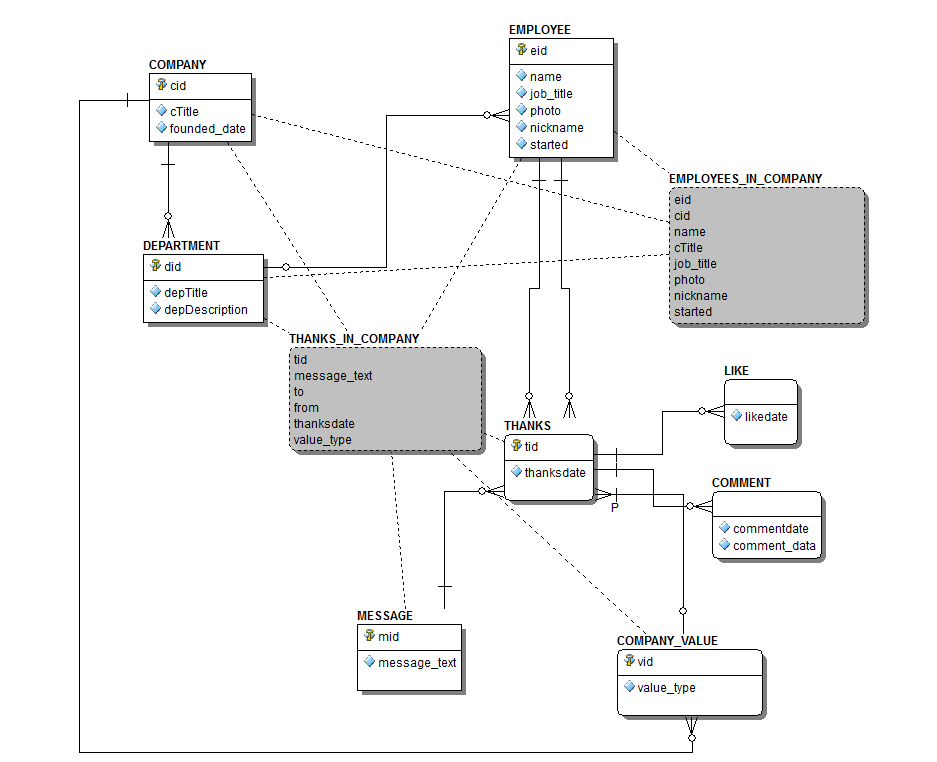
\includegraphics[scale=.7]{./images/erd12-5.PNG}
\end{figure}
\clearpage

\section{Conceptual Model of the Enterprise}
A conceptual model of the Thanks database. \\

company(\underline{cid}, cTitle, founded\_date) \\
PK - cid \\
CK - cid, cTitle \\
AK - cTitle \\

department(\underline{did}, depTitle, depDescription) \\
PK - did \\
CK - did \\
FK - department.headid REFERENCES departmenthead.headid \\
     department.cid REFERENCES company.cid \\

employee(\underline{eid}, name, job\_title, photo, nickname, started) \\
PK - eid \\
CK - eid, name, photo \\
AK - name, photo \\
FK - employee.did REFERENCES department.did \\

thanks(\underline{(tid, mid)}, thanksdate) \\
PK - (tid, mid) \\
CK - tid \\
FK - thanks.mid REFERENCES message.mid \\
     thanks.to REFERENCES employee.eid \\
     thanks.from REFERENCES employee.eid \\
     thanks.vid REFERENCES company\_value.vid \\

like(\underline{(likeid, tid)}, likedate) \\
PK - (likeid, tid) \\
CK - likeid \\
FK - like.tid REFERENCES thanks.tid \\

comment(\underline{(commentid, tid)}, comment\_data, commentdate) \\
PK - (commentid, tid) \\
CK - commentid \\
FK - comment.tid REFERENCES thanks.tid \\

message(\underline{mid}, message\_text) \\
PK - mid \\
CK - mid \\

company\_value(\underline{vid}, value\_type) \\
PK - vid \\
CK - vid \\
FK - company\_value.cid REFERENCES company.cid
\clearpage
\section{Table Dictionary}
\begin{table}[h]
\centering
\resizebox{\textwidth}{!}{%
\begin{tabular}{|p{5cm}|p{5cm}|p{5cm}|}

\hline
\multicolumn{1}{|c|}{\textbf{Table}} & \multicolumn{1}{c|}{\textbf{Attributes}}                            & \multicolumn{1}{c|}{\textbf{Definition}}               \\ \hline
COMPANY                              & cid, cTitle, founded\_date                                          & Represents a company, which is the starting data point \\ \hline
DEPARTMENT                           & did, depTitle, depDescription, headid, cid                          & Department in a company                                \\ \hline
EMPLOYEE                             & \underline{eid}, name, job\_title, photo, nickname, started, did    & Employee in a company                                  \\ \hline
THANKS                               & tid, thanksdate                                                     & Data type used to recognize another employee           \\ \hline
LIKE                                 & likeid, tid, likedate                                               & A like on a Thanks post                                \\ \hline
COMMENT                              & commentid, tid, commentdate, comment\_data                              & A comment on a Thanks post                             \\ \hline
MESSAGE                              & mid, message\_text                                                  & Message of a Thanks                                    \\ \hline
COMPANY\_VALUE                       & vid, value\_type                                                    & Company value of a Thanks                              \\ \hline
EMPLOYEES\_IN\_COMPANY               & eid, cid, name, cTitle, job\_title, photo, nickname, started                                                    & View of employees and their respective companies                              \\ \hline
THANKS\_IN\_COMPANY                  & tid, message\_text, to, from, thanksdate, value\_type                                                   & View of Thanks and their respective attributes                             \\ \hline
\end{tabular}
}
\end{table}
\clearpage
\section{Attribute Dictionary}
\begin{table}[h]
\centering
\resizebox{\textwidth}{!}{%
\begin{tabular}{|l|l|l|}

\hline
\multicolumn{1}{|c|}{\textbf{Attribute}} & \multicolumn{1}{c|}{\textbf{Tables Used In}} & \multicolumn{1}{c|}{\textbf{Description}}        \\ \hline
eid                                      & EMPLOYEE, EMPLOYEES\_IN\_COMPANY             & Unique identifier of an employee                 \\ \hline
name                                     & EMPLOYEE, EMPLOYEES\_IN\_COMPANY             & Name of an employee                              \\ \hline
job\_title                               & EMPLOYEE, EMPLOYEES\_IN\_COMPANY             & Job title of employee                            \\ \hline
photo                                    & EMPLOYEE, EMPLOYEES\_IN\_COMPANY             & Photo of employee                                \\ \hline
nickname                                 & EMPLOYEE, EMPLOYEES\_IN\_COMPANY             & Nickname of employee                             \\ \hline
started                                  & EMPLOYEE, EMPLOYEES\_IN\_COMPANY             & Date that the employee started at their company  \\ \hline
did                                      & DEPARTMENT                                   & Unique identifier of the department of a company \\ \hline
depTitle                                 & DEPARTMENT                                   & Name (title) of the department                   \\ \hline
depDescription                           & DEPARTMENT                                   & Description of the department                    \\ \hline
cid                                      & COMPANY, EMPLOYEES\_IN\_COMPANY              & Unique identifier of a company                   \\ \hline
cTitle                                   & COMPANY, EMPLOYEES\_IN\_COMPANY              & Name (title) of a company                        \\ \hline
founded\_date                            & COMPANY                                      & Date a company was founded                       \\ \hline
tid                                      & THANKS, THANKS\_IN\_COMPANY                  & Unique identifier of a Thanks                    \\ \hline
thanksdate                               & THANKS, THANKS\_IN\_COMPANY                  & Date the Thanks was given                        \\ \hline
likeid                                   & LIKE                                         & Unique identifier of a like on a Thanks          \\ \hline
likedate                                 & LIKE                                         & Date the like was given                          \\ \hline
commentid                                & COMMENT                                      & Unique identifier of a comment                   \\ \hline
comment\_data                            & COMMENT                                      & Message of comment                    \\ \hline
commentdate                              & COMMENT                                      & Date the comment was added to the Thanks         \\ \hline
mid                                      & MESSAGE                                      & Unique identifier of the message of a Thanks     \\ \hline
message\_text                            & MESSAGE, THANKS\_IN\_COMPANY                 & Body text of the message of a Thanks             \\ \hline
vid                                      & COMPANY\_VALUE                               & Unique identifier of a company value             \\ \hline
value\_type                              & COMPANY\_VALUE, THANKS\_IN\_COMPANY          & Name (type) of company value                     \\ \hline
\end{tabular}
}
\end{table}
\clearpage

\chapter{Database and Query Definition}

\section{Database Definition}
\verbatiminput{sql/ThanksCorporation.sql}
\section{Database Queries}
Given below are 14 example English queries, with their SQL DML used to retrieve the necessary data.
\begin{enumerate}
    \item List the names of all employees in the company ``I Love Thanks".
    \begin{verbatim}
    SELECT name
    FROM   EMPLOYEES_IN_COMPANY
    WHERE  cTitle = "I Love Thanks"
    ;
    \end{verbatim}
    \item Show all department names in the corporation ``Blitz''.
    \begin{verbatim}
    SELECT d.depTitle
    FROM COMPANY AS c
        INNER JOIN DEPARTMENT AS d ON c.cid = d.cid
    WHERE c.cTitle = "Blitz"
    ;
    \end{verbatim}
    \item Return a list of all employees in the database who have nicknames.
    \begin{verbatim}
    SELECT e.nickname
         , e.name
    FROM EMPLOYEE AS e
    WHERE e.nickname IS NOT NULL
    ;
    \end{verbatim}
    \item Show names of employees who do not have photos in the ``I Love Thanks" company.
    \begin{verbatim}
    SELECT e.name
    FROM COMPANY AS c
        INNER JOIN DEPARTMENT AS d ON c.cid = d.cid
        INNER JOIN EMPLOYEE   AS e ON d.did = e.did
    WHERE e.photo IS NULL
        AND c.cTitle = "I Love Thanks"
    ;
    \end{verbatim}
    \item Show all comments on Julia Crow's Thanks to Richard Baker on January 2, 2011.
    \begin{verbatim}
    SELECT commentdate
         , comment_data
    FROM COMMENT
    WHERE tid = (
        SELECT t.tid
        FROM THANKS_IN_COMPANY AS t
        WHERE t.to = (
            SELECT eid
            FROM   EMPLOYEES_IN_COMPANY
            WHERE  name = "Richard Baker"
        )
        AND t.from = (
            SELECT eid
            FROM   EMPLOYEES_IN_COMPANY
            WHERE  name = "Julia Crow"
        )
        AND t.thanksdate = "2011-1-2"
    )
    ;
    \end{verbatim}
    \item Show all of the Thanks that Julia Crow from ``First America'' gave.
    \begin{verbatim}
    SELECT thanks.`from`
         , addressed_to.name as `to`
         , thanks.message
         , thanks.thanksdate
         , thanks.value
    FROM (
        SELECT e.name AS `from`
             , t.`to`
             , m.message_text AS message
             , t.thanksdate
             , cv.value_type AS value
        FROM COMPANY AS c
            INNER JOIN DEPARTMENT    AS d  ON c.cid    = d.cid
            INNER JOIN EMPLOYEE      AS e  ON d.did    = e.did
            INNER JOIN THANKS        AS t  ON t.`from` = e.eid
            INNER JOIN MESSAGE       AS m  ON t.mid    = m.mid
            INNER JOIN COMPANY_VALUE AS cv ON t.vid    = cv.vid
        WHERE c.cTitle = "First America"
            AND e.name = "Julia Crow"
    ) AS thanks
    , EMPLOYEE AS addressed_to
    WHERE addressed_to.eid = thanks.`to`
    ;
    \end{verbatim}
    \item Show all of the Thanks that Emma Cross from ``Lightning Corporation'' received.
    \begin{verbatim}
    SELECT thanks.`to`
         , addressed_to.name AS `from`
         , thanks.message
         , thanks.thanksdate
         , thanks.value
    FROM (
        SELECT e.name as `to`
             , t.`from`
             , m.message_text AS message
             , t.thanksdate
             , cv.value_type AS value
        FROM COMPANY AS c
            INNER JOIN DEPARTMENT    AS d  ON c.cid  = d.cid
            INNER JOIN EMPLOYEE      AS e  ON d.did  = e.did
            INNER JOIN THANKS        AS t  ON t.`to` = e.eid
            INNER JOIN MESSAGE       AS m  ON t.mid  = m.mid
            INNER JOIN COMPANY_VALUE AS cv ON t.vid  = cv.vid
        WHERE c.cTitle = "Lightning Corporation"
            AND e.name = "Emma Cross"
    ) AS thanks
    , EMPLOYEE as addressed_to
    WHERE addressed_to.eid = thanks.`from`
    ;
    \end{verbatim}
    \item Show all thanks that have been given in the corporation ``First America'' before 2013.
    \begin{verbatim}
    SELECT t.to
         , t.from
         , m.message_text
         , t.thanksdate
         , cv.value_type
    FROM COMPANY AS c
        INNER JOIN DEPARTMENT    AS d  ON c.cid  = d.cid
        INNER JOIN EMPLOYEE      AS e  ON d.did  = e.did
        INNER JOIN THANKS        AS t  ON t.`to` = e.eid
        INNER JOIN COMPANY_VALUE AS cv ON t.vid  = cv.vid
        INNER JOIN MESSAGE       AS m  ON t.mid  = m.mid
    WHERE c.cTitle = "First America"
        AND t.thanksdate < '2013-1-1'
    ;
    \end{verbatim}
    \item List the company values of ``Blitz''.
    \begin{verbatim}
    SELECT cv.value_type
    FROM   COMPANY AS c
        INNER JOIN COMPANY_VALUE as cv on c.cid = cv.cid
    WHERE  c.cTitle = "Blitz"
    ;
    \end{verbatim}
    \item Who is the newest employee to have joined the company ``Lightning Corporation''?
    \begin{verbatim}
    SELECT e.name
    FROM COMPANY AS c
        INNER JOIN DEPARTMENT AS d ON c.cid = d.cid
        INNER JOIN EMPLOYEE   AS e ON d.did = e.did
    WHERE c.cTitle = "Lightning Corporation"
        AND e.started = (
            SELECT MAX(e.started)
            FROM COMPANY AS c
                INNER JOIN DEPARTMENT AS d ON c.cid = d.cid
                INNER JOIN EMPLOYEE   AS e ON d.did = e.did
            WHERE c.cTitle = "Lightning Corporation"
        )
    ;
    \end{verbatim}
    \item List all Thanks ``I Love Thanks'' employees gave in October 2011.
    \begin{verbatim}
    SELECT t.to
         , t.from
         , m.message_text
         , t.thanksdate
         , cv.value_type
    FROM COMPANY AS c
        INNER JOIN DEPARTMENT    AS d  ON c.cid  = d.cid
        INNER JOIN EMPLOYEE      AS e  ON d.did  = e.did
        INNER JOIN THANKS        AS t  ON t.`to` = e.eid
        INNER JOIN COMPANY_VALUE AS cv ON t.vid  = cv.vid
        INNER JOIN MESSAGE       AS m  ON t.mid  = m.mid
    WHERE MONTHNAME(t.thanksdate) = "October"
        AND YEAR(t.thanksdate) = 2011
    ;
    \end{verbatim}
    \item Find the name of the employee who received the most Thanks in ``Blitz''.
    \begin{verbatim}
    SELECT e.name
    FROM COMPANY AS c
        INNER JOIN DEPARTMENT AS d ON c.cid = d.cid
        INNER JOIN EMPLOYEE   AS e ON d.did = e.did
        INNER JOIN THANKS     AS t ON t.to  = e.eid
    WHERE c.cTitle = "Blitz"
        AND t.to = (
            SELECT `to` FROM (
                SELECT `to`, count(`to`) AS counted
                FROM COMPANY AS c
                    INNER JOIN DEPARTMENT AS d ON c.cid = d.cid
                    INNER JOIN EMPLOYEE   AS e ON d.did = e.did
                    INNER JOIN THANKS     AS t ON t.to  = e.eid
                WHERE c.cTitle = "Blitz"
                GROUP BY `to`
                ORDER BY counted DESC
                LIMIT 1
            ) as received_most_thanks
        )
        GROUP BY `to`
    ;
    \end{verbatim}
    \item Find the average number of likes each Thanks in the corporation ``Blitz'' received in 2011.
    \begin{verbatim}
    SELECT AVG(avg.counter) as average
    FROM (
        SELECT l.tid, count(l.likeid) as counter
        FROM COMPANY AS c
            INNER JOIN DEPARTMENT AS d ON c.cid = d.cid
            INNER JOIN EMPLOYEE   AS e ON d.did = e.did
            INNER JOIN THANKS     AS t ON t.to  = e.eid
            INNER JOIN `LIKE`     AS l ON t.tid = l.tid
        WHERE c.cTitle = "Blitz"
        AND   YEAR(t.thanksdate) = 2011
        GROUP BY l.tid
    ) AS avg
    ;
    \end{verbatim}
    \item Find the most awarded company value in ``Blitz''.
    \begin{verbatim}
    SELECT cv.value_type
    FROM COMPANY AS c
        INNER JOIN DEPARTMENT    AS d  ON c.cid = d.cid
        INNER JOIN EMPLOYEE      AS e  ON d.did = e.did
        INNER JOIN THANKS        AS t  ON e.eid = t.to
        INNER JOIN COMPANY_VALUE AS cv ON t.vid = cv.vid
    WHERE c.cTitle = "Blitz"
    GROUP BY value_type
    ORDER BY COUNT(VALUE_TYPE) DESC
    LIMIT 1
    ;
    \end{verbatim}
\end{enumerate}
\section{Design Tradeoffs and Limitations}

One of the biggest design tradeoffs is that an employee can only be associated with one company. This can become difficult if an employee leaves a company and wants to take their data with them to a new company. An example of this can be seen more clearly when the attribute ``started'' is taken into account. If an employee is starting in a new position, this date has to change and is no longer preserved. However, since the idea of Thanks Corporation is to maintain a private way to share Thanks within a company, this seemed to be a fair tradeoff. The ``started'' example is a more difficult limitation of the database, but necessary without another entity. \\

Another tradeoff of the database is the lack of multiple job titles. Multiple photos are also not allowed, so if transferring between companies were ever a feature in the future, these would not work in a future implementation. Another design limitation is the lack of Thanks being given between corporations. Since I wanted to keep the database as small communities of corporations rather than one large social network, it seemed to be the right tradeoff.
\clearpage

\chapter{Database Integrity and Security}

\section{Functional Dependencies}
\begin{itemize}
\item cid $\rightarrow$ cTitle, founded\_date
\item did $\rightarrow$ depTitle, depDescription
\item eid $\rightarrow$ name, job\_title, photo, nickname, started
\item tid $\rightarrow$ thanksdate
\item likeid $\rightarrow$ likedate
\item commentid $\rightarrow$ comment\_data, commentdate
\item mid $\rightarrow$ message\_text
\item vid $\rightarrow$ value\_type
\end{itemize}
\section{Adjustments for Normalization}
According to these functional dependencies and after looking at the ERD, it is clear that the database has already been normalized. Therefore, no adjustments will be needed on top of what already is in normalizing this database.
\section{Integrity and Security}
\begin{enumerate}
\item Users and Granted Privileges\\
There will multiple types of access privileges to the database. These access types are listed below.
    \begin{itemize}
    \item Webmaster User \\
    A webmaster represents access privileges for the owner of Thanks Corporation. He has complete access to all data at any time.
    \item Executive User \\
    Allows access to an executive's own company entity, and allows for modification of its attributes.
    \item Department Head User \\
    Allows access to a department head's own department entity, and allows for modification of its attributes.
    \item Employee User \\
    Allows normal access for an employee: modification of own employee entity and insert/update/delete privileges for own Thanks and related entities.
    \end{itemize}
\item Assertion \\
MySQL does not directly provide assertions, however triggers have been used to provide assertion-like functionality in MySQL. Assertions the Thanks Corporation needs are listed below.
    \begin{itemize}
    \item Determine whether an employee giving a Thanks with a company value is using a company value from the employee's own company.
    \end{itemize}
\item Views \\
Two views are utilized in this database.
    \begin{itemize}
    \item EMPLOYEES\_IN\_COMPANY \\
    Returns employees from all departments associated with a company.
    \item THANKS\_IN\_COMPANY \\
    Returns all thanks from within a company.
    \end{itemize}
\end{enumerate}
\clearpage
\chapter{Implementation Notes}
\section{Indices}
Refer to section IV.1 for a list of used indices.
\section{Data}
\verbatiminput{sql/ThanksCorpDataLoad.sql}
\section{Query Trace}
A query trace is found on the next page.
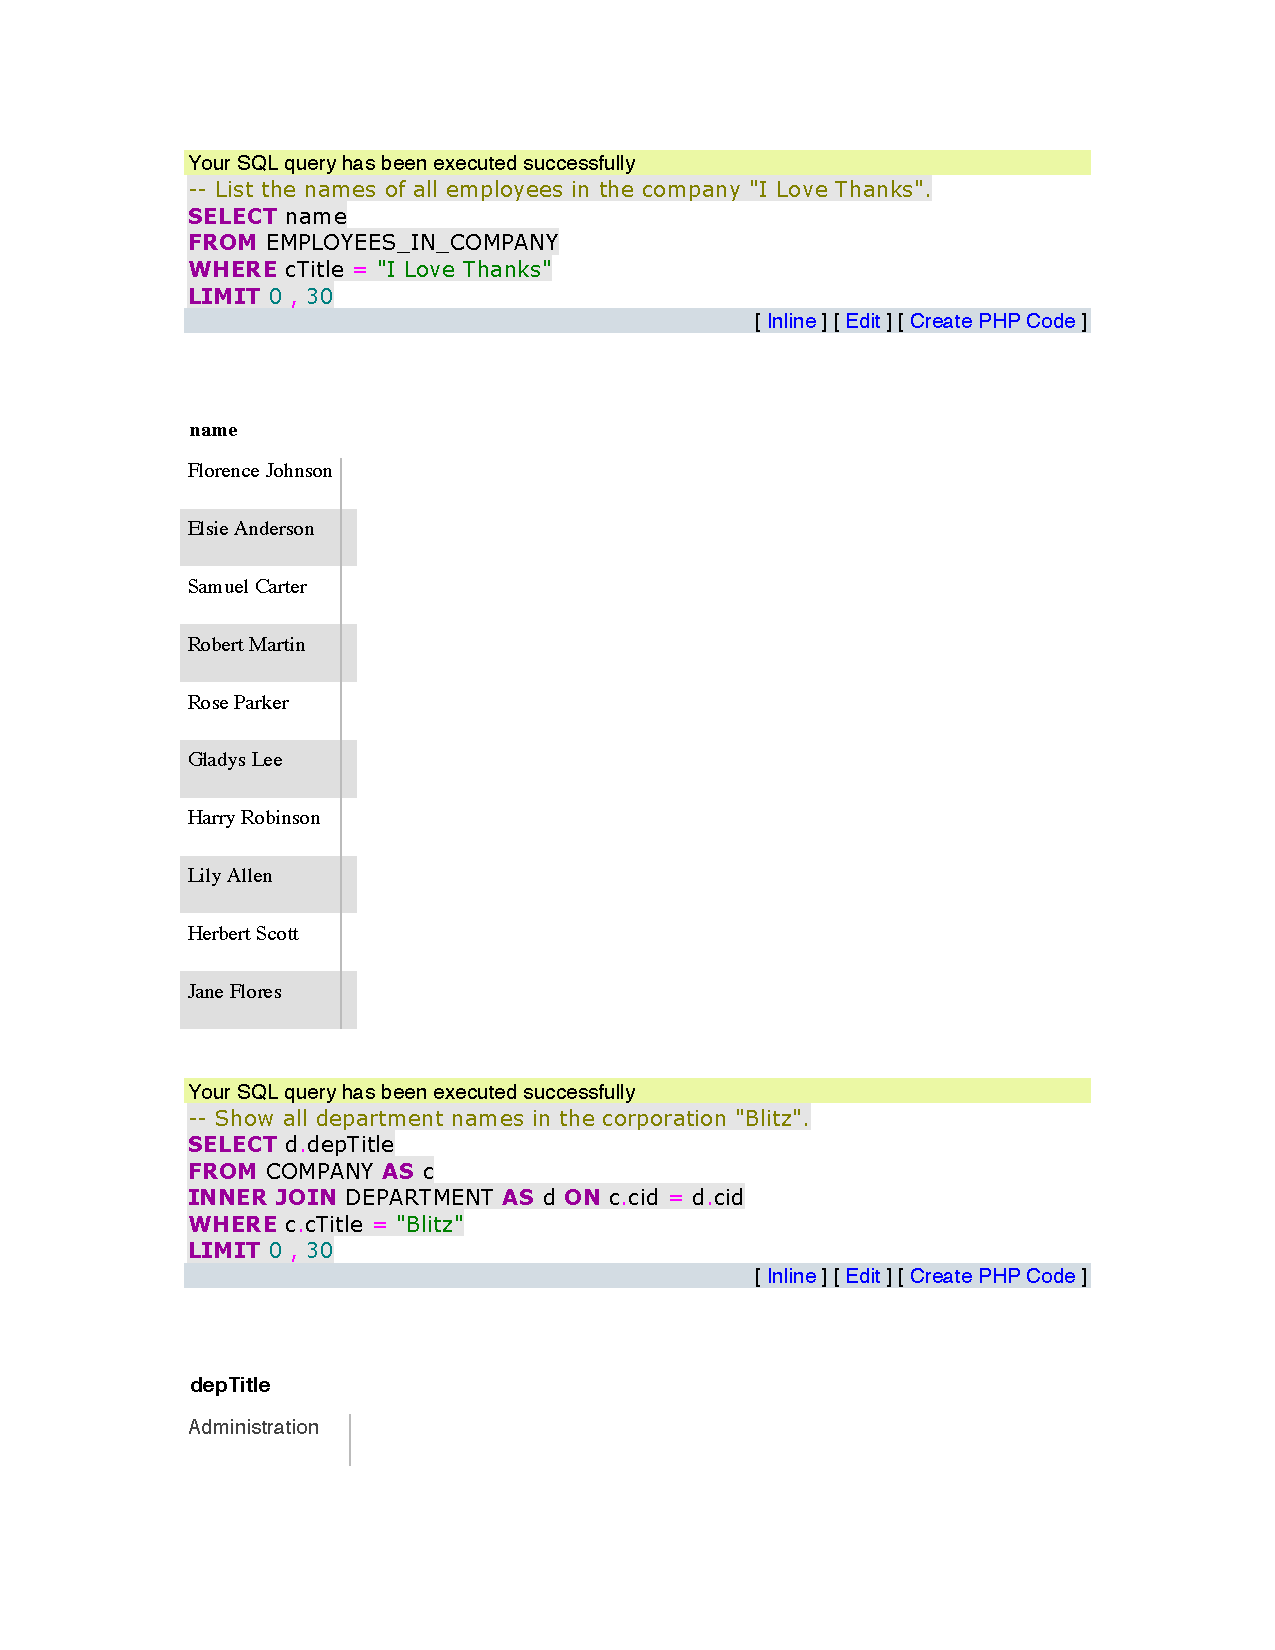
\includepdf[pages={1-8}]{query-trace.pdf}
\section{Implementation Assessment}
I had to adjust some of the data types, as my primary keys were not autoincrementing when I inserted new data. I also switched datetime to date for a few data types in order to maintain some consistency. Finally, I modified a database relation since it was conflicting with what I wanted. Overall, after those fixes all of the implementations went smoothly and I was able to get my query trace up and running quickly.
\chapter{Lessons Learned}
\indent % Would not indent first paragraph without.
\indent One thing I would do differently if I approached the project again would be to put more effort into concepting the initial idea. Instead of depending on revisions in order to hash out a good database design, I should have made an effort to expand my knowledge and find good examples of how to represent my entities and relationships before assuming they were right. While I was able to come up with a solid database design, it ended up taking much longer and required a few hours extra spent on database design later on in the project. I would also start the project working in LaTeX and ER Studio from the beginning. I ended up dividing the information in my deliverables, and towards the fourth deliverable it became difficult to manage all of the different sections and edit my information accordingly. In regards to ER Studio, I eventually had to transcribe my entity-relationship diagram anyways in order to cut down on the time needed to write the SQL code. It also provided a nice diagram for my project section, which I would have had to hand-draw otherwise. While these two things were extremely difficult in the beginning of the project, by the time I reached the fifth and sixth deliverable I found my adjustments to be way less challenging, especially with the project all in one document. \\
\indent For time spent on the project, I probably spent somewhere between fifty and sixty hours on the project. As I mentioned in my difficulties in the project, I also ended up migrating the database project into LaTeX. This took much longer than expected due to my lack of experience and lack of examples, so approximately five of these hours were spent in formatting alone. Additional time beyond this initial setup was spent in figuring out table formatting and resizing. However, I found this to be time well spent. Moving to LaTeX allowed me to improve my workflow in later deliverables, and helped me worry less about my formatting. Overall, I believe I spent a fair amount of time on the project considering the constraints of time from other classes, such as the Group Senior Project course. \\
\indent The project was useful in helping me learn the course material in a few ways. Writing the database queries necessary for my database improved my SQL query knowledge. As for completing the project and turning it into a production environment, several things need to be considered. The lack of true assertions in MySQL make it difficult to validate data, which requires a great deal of validation work to be done server side before the INSERT queries are made. In addition, there are some tradeoffs to the database design, such as employees being exclusive to one company, which would complicate things for a server and client when an employee moves to a different company. Finally, adding more views would make it easier to access the necessary data a client needs to display information for this corporation. \\
\indent Overall, I learned a lot through the project and had a great time realizing Thanks Corporation in MySQL.

\end{document}
